%%%%%%%%%%%%%%%%%%%%%%%
% Comp 160, Fall 2019
% Homework 3
% Author: Vladimir Hugec
%%%%%%%%%%%%%%%%%%%%%%%

% This portion of the LaTeX document are configuration 
% You can see it as all the #includes in C++
\documentclass[12pt]{article}

\usepackage{epsfig}
\usepackage{amsmath}
\usepackage{amsthm}
\usepackage{listings}
\usepackage{graphicx}
\usepackage{tikz}

\newtheorem{lemma}{Lemma}
\newtheorem{theorem}{Theorem}

\usepackage{titlesec}
\titleformat{\section}
{\normalfont\Large\bfseries}{Question~\thesection:}{1em}{}

\newlength{\toppush}
\setlength{\toppush}{2\headheight}
\addtolength{\toppush}{\headsep}

\def\subjnum{Comp 160}
\def\subjname{Introduction to Algorithms}

\def\doheading#1#2#3{\vfill\eject\vspace*{-\toppush}%
  \vbox{\hbox to\textwidth{{\bf} \subjnum: \subjname \hfil Vladimir Hugec}%
    \hbox to\textwidth{{\bf} Tufts University, Fall 2019 \hfil#3\strut}%
    \hrule}}


\newcommand{\htitle}[1]{\vspace*{1.25ex plus 1ex minus 0ex}%
\begin{center}
{\large\bf #1}
\end{center}} 


%%%%%%%%%%%%%%%%%%%%%%%%%%%%%%%%%%%%%%%%%%%%%%%%%%%%%%%%%%%%%%%%%%%
% BEGIN DOCUMENT
%%%%%%%%%%%%%%%%%%%%%%%%%%%%%%%%%%%%%%%%%%%%%%%%%%%%%%%%%%%%%%%%%%%
\begin{document}
\doheading{2}{title}{Homework 3}

\section{Median of n values using groups}
\subsection{K groups}

\begin{lemma}
If we have groups of $k$, in each iteration we can remove at least $\frac{n}{k}$ elements.
\end{lemma}
\begin{proof}


$\newline$ K-rows$\left\{\begin{array}{ccccc}0 & 0 & 0 & 0 & 0 \\0 & 0 & 0 & 0 & 0 \\0 & 0 & X & 0 & 0 \\... & ... & ... & ... & ... \\0 & 0 & 0 & 0 & 0\end{array}\right.$

$\newline$ Following the steps in the algorithm covered in class:

i. Form $\frac{n}{k}$ groups of $k$ elements. ( O(n) )

ii. Find the median of each group. ( O (n) )

iii. Recursively find the median among all group medians ( T($\lceil \frac{n}{k} \rceil$) )

iv. Partition around x. ( O(n) )

v. If rank(x) is not the target rank, recurse on the subset of elements that contains the target rank.

$\newline$ To figure out the time complexity of step v, we look at the subsets included in the recursion in the worst case. (Assuming $n$ is divisible by $k$ for simplicity). We start with $n$ elements, and since we are sorting in groups of $k$ we know that there are $\frac{n}{k}$ columns. Since these rows and columns are sorted already in a way that the elements to the lower left of our median of medians (X in the diagram) all must be less than X, and the elements to the upper right all must be greater than X. Assuming $k \geq 6$, we know that at worst case our recursion will be:

\begin{center}
$n - (\frac{n}{k}) = \frac{nk}{k} - \frac{n}{k} = \frac{nk - n}{k} = \frac{n(k - 1)}{k}$
\end{center}

Therefore the worst case time complexity for step v. is T($\frac{n(k - 1)}{k}$). Which means that:

\begin{center}
$T(n) = \Theta(n) + T(\frac{n}{k}) + T(\frac{n(k - 1)}{k})$
\end{center}

\end{proof}

\subsection{Modifying K}

If we suppose one really large K, 1,000,000, and one relatively small, 100, modifying the constant K with a smaller value, as noted in the recitation notes, will increase the runtime of the algorithm. Thus it follows that when implementing the algorithm, the larger the K, the more efficient the algorithm. I suggest that a K value of 1,000,000 should be used.


\pagebreak

\section{Algorithm}

\includegraphics[scale=0.74]{algo}

\pagebreak

\section{Heaps}
\subsection{Min-Heap Bottom Up}

\begin{center}
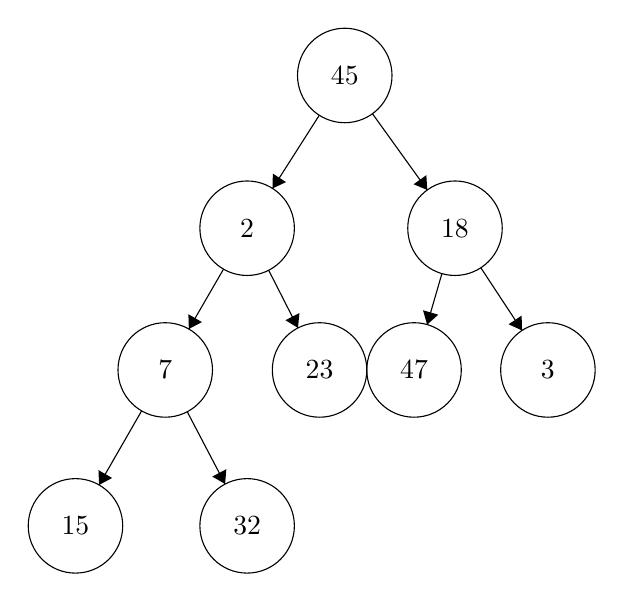
\begin{tikzpicture}[scale=0.2]
\tikzstyle{every node}+=[inner sep=0pt]
\draw [black] (38,-6.6) circle (3);
\draw (38,-6.6) node {$45$};
\draw [black] (31.8,-16.3) circle (3);
\draw (31.8,-16.3) node {$2$};
\draw [black] (45,-16.3) circle (3);
\draw (45,-16.3) node {$18$};
\draw [black] (26.6,-25.3) circle (3);
\draw (26.6,-25.3) node {$7$};
\draw [black] (36.4,-25.3) circle (3);
\draw (36.4,-25.3) node {$23$};
\draw [black] (42.4,-25.3) circle (3);
\draw (42.4,-25.3) node {$47$};
\draw [black] (50.9,-25.3) circle (3);
\draw (50.9,-25.3) node {$3$};
\draw [black] (20.9,-35.2) circle (3);
\draw (20.9,-35.2) node {$15$};
\draw [black] (31.8,-35.2) circle (3);
\draw (31.8,-35.2) node {$32$};
\draw [black] (36.38,-9.13) -- (33.42,-13.77);
\fill [black] (33.42,-13.77) -- (34.27,-13.37) -- (33.43,-12.83);
\draw [black] (39.76,-9.03) -- (43.24,-13.87);
\fill [black] (43.24,-13.87) -- (43.18,-12.93) -- (42.37,-13.51);
\draw [black] (30.3,-18.9) -- (28.1,-22.7);
\fill [black] (28.1,-22.7) -- (28.93,-22.26) -- (28.07,-21.76);
\draw [black] (33.17,-18.97) -- (35.03,-22.63);
\fill [black] (35.03,-22.63) -- (35.12,-21.69) -- (34.23,-22.14);
\draw [black] (44.17,-19.18) -- (43.23,-22.42);
\fill [black] (43.23,-22.42) -- (43.94,-21.79) -- (42.97,-21.51);
\draw [black] (46.64,-18.81) -- (49.26,-22.79);
\fill [black] (49.26,-22.79) -- (49.23,-21.85) -- (48.4,-22.4);
\draw [black] (25.1,-27.9) -- (22.4,-32.6);
\fill [black] (22.4,-32.6) -- (23.23,-32.16) -- (22.36,-31.66);
\draw [black] (28,-27.96) -- (30.4,-32.54);
\fill [black] (30.4,-32.54) -- (30.48,-31.6) -- (29.59,-32.07);
\end{tikzpicture}

$\downarrow$
\end{center}

\begin{center}
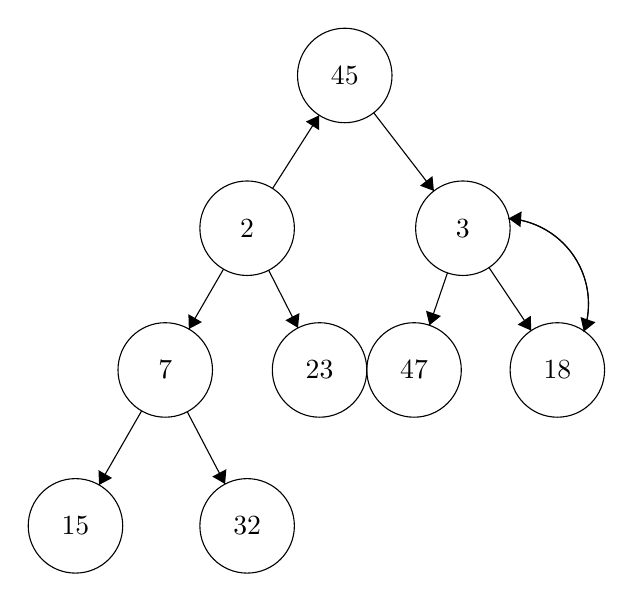
\begin{tikzpicture}[scale=0.2]
\tikzstyle{every node}+=[inner sep=0pt]
\draw [black] (38,-6.6) circle (3);
\draw (38,-6.6) node {$45$};
\draw [black] (31.8,-16.3) circle (3);
\draw (31.8,-16.3) node {$2$};
\draw [black] (45.5,-16.3) circle (3);
\draw (45.5,-16.3) node {$3$};
\draw [black] (26.6,-25.3) circle (3);
\draw (26.6,-25.3) node {$7$};
\draw [black] (36.4,-25.3) circle (3);
\draw (36.4,-25.3) node {$23$};
\draw [black] (42.4,-25.3) circle (3);
\draw (42.4,-25.3) node {$47$};
\draw [black] (51.5,-25.3) circle (3);
\draw (51.5,-25.3) node {$18$};
\draw [black] (20.9,-35.2) circle (3);
\draw (20.9,-35.2) node {$15$};
\draw [black] (31.8,-35.2) circle (3);
\draw (31.8,-35.2) node {$32$};
\draw [black] (39.84,-8.97) -- (43.66,-13.93);
\fill [black] (43.66,-13.93) -- (43.57,-12.99) -- (42.78,-13.6);
\draw [black] (30.3,-18.9) -- (28.1,-22.7);
\fill [black] (28.1,-22.7) -- (28.93,-22.26) -- (28.07,-21.76);
\draw [black] (33.17,-18.97) -- (35.03,-22.63);
\fill [black] (35.03,-22.63) -- (35.12,-21.69) -- (34.23,-22.14);
\draw [black] (44.52,-19.14) -- (43.38,-22.46);
\fill [black] (43.38,-22.46) -- (44.11,-21.87) -- (43.16,-21.54);
\draw [black] (25.1,-27.9) -- (22.4,-32.6);
\fill [black] (22.4,-32.6) -- (23.23,-32.16) -- (22.36,-31.66);
\draw [black] (28,-27.96) -- (30.4,-32.54);
\fill [black] (30.4,-32.54) -- (30.48,-31.6) -- (29.59,-32.07);
\draw [black] (33.42,-13.77) -- (36.38,-9.13);
\fill [black] (36.38,-9.13) -- (35.53,-9.53) -- (36.37,-10.07);
\draw [black] (48.397,-15.683) arc (86.21865:-18.83851:5.437);
\fill [black] (53.18,-22.86) -- (53.92,-22.27) -- (52.97,-21.94);
\draw [black] (48.396,-15.68) arc (86.27406:-18.89393:5.436);
\fill [black] (48.4,-15.68) -- (49.16,-16.23) -- (49.23,-15.23);
\draw [black] (47.16,-18.8) -- (49.84,-22.8);
\fill [black] (49.84,-22.8) -- (49.81,-21.86) -- (48.98,-22.42);
\end{tikzpicture}

$\downarrow$

\end{center}
\begin{center}
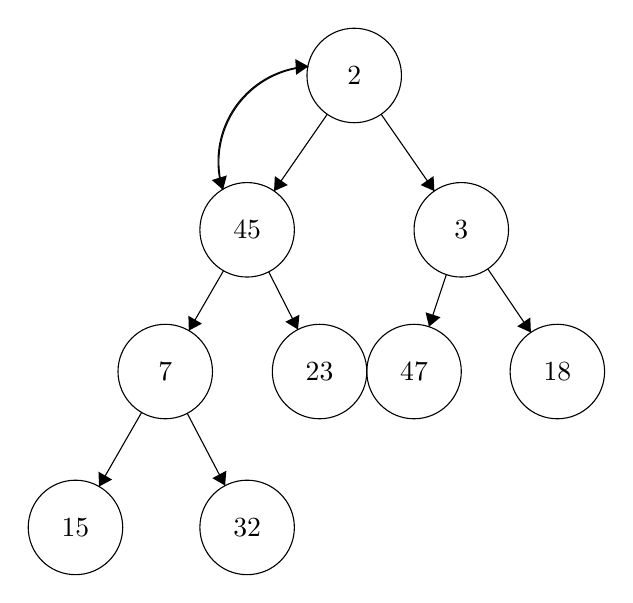
\begin{tikzpicture}[scale=0.2]
\tikzstyle{every node}+=[inner sep=0pt]
\draw [black] (38.6,-6.5) circle (3);
\draw (38.6,-6.5) node {$2$};
\draw [black] (31.8,-16.3) circle (3);
\draw (31.8,-16.3) node {$45$};
\draw [black] (45.4,-16.3) circle (3);
\draw (45.4,-16.3) node {$3$};
\draw [black] (26.6,-25.3) circle (3);
\draw (26.6,-25.3) node {$7$};
\draw [black] (36.4,-25.3) circle (3);
\draw (36.4,-25.3) node {$23$};
\draw [black] (42.4,-25.3) circle (3);
\draw (42.4,-25.3) node {$47$};
\draw [black] (51.5,-25.3) circle (3);
\draw (51.5,-25.3) node {$18$};
\draw [black] (20.9,-35.2) circle (3);
\draw (20.9,-35.2) node {$15$};
\draw [black] (31.8,-35.2) circle (3);
\draw (31.8,-35.2) node {$32$};
\draw [black] (40.31,-8.96) -- (43.69,-13.84);
\fill [black] (43.69,-13.84) -- (43.64,-12.89) -- (42.82,-13.46);
\draw [black] (30.3,-18.9) -- (28.1,-22.7);
\fill [black] (28.1,-22.7) -- (28.93,-22.26) -- (28.07,-21.76);
\draw [black] (33.17,-18.97) -- (35.03,-22.63);
\fill [black] (35.03,-22.63) -- (35.12,-21.69) -- (34.23,-22.14);
\draw [black] (44.45,-19.15) -- (43.35,-22.45);
\fill [black] (43.35,-22.45) -- (44.08,-21.85) -- (43.13,-21.54);
\draw [black] (25.1,-27.9) -- (22.4,-32.6);
\fill [black] (22.4,-32.6) -- (23.23,-32.16) -- (22.36,-31.66);
\draw [black] (28,-27.96) -- (30.4,-32.54);
\fill [black] (30.4,-32.54) -- (30.48,-31.6) -- (29.59,-32.07);
\draw [black] (30.236,-13.776) arc (-162.43778:-267.07405:6.042);
\fill [black] (35.69,-5.92) -- (34.86,-5.46) -- (34.91,-6.46);
\draw [black] (47.08,-18.78) -- (49.82,-22.82);
\fill [black] (49.82,-22.82) -- (49.78,-21.87) -- (48.95,-22.43);
\draw [black] (30.267,-13.757) arc (-163.11224:-266.39958:6.056);
\fill [black] (30.27,-13.76) -- (30.51,-12.85) -- (29.56,-13.14);
\draw [black] (36.89,-8.96) -- (33.51,-13.84);
\fill [black] (33.51,-13.84) -- (34.38,-13.46) -- (33.56,-12.89);
\end{tikzpicture}

$\downarrow$
\end{center}

\begin{center}
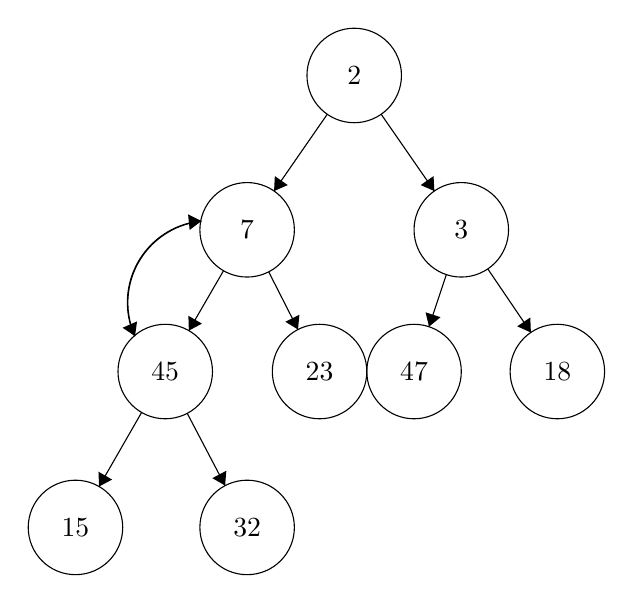
\begin{tikzpicture}[scale=0.2]
\tikzstyle{every node}+=[inner sep=0pt]
\draw [black] (38.6,-6.5) circle (3);
\draw (38.6,-6.5) node {$2$};
\draw [black] (31.8,-16.3) circle (3);
\draw (31.8,-16.3) node {$7$};
\draw [black] (45.4,-16.3) circle (3);
\draw (45.4,-16.3) node {$3$};
\draw [black] (26.6,-25.3) circle (3);
\draw (26.6,-25.3) node {$45$};
\draw [black] (36.4,-25.3) circle (3);
\draw (36.4,-25.3) node {$23$};
\draw [black] (42.4,-25.3) circle (3);
\draw (42.4,-25.3) node {$47$};
\draw [black] (51.5,-25.3) circle (3);
\draw (51.5,-25.3) node {$18$};
\draw [black] (20.9,-35.2) circle (3);
\draw (20.9,-35.2) node {$15$};
\draw [black] (31.8,-35.2) circle (3);
\draw (31.8,-35.2) node {$32$};
\draw [black] (40.31,-8.96) -- (43.69,-13.84);
\fill [black] (43.69,-13.84) -- (43.64,-12.89) -- (42.82,-13.46);
\draw [black] (24.677,-23.051) arc (-155.97821:-264.05853:5.204);
\fill [black] (24.68,-23.05) -- (24.81,-22.12) -- (23.89,-22.52);
\draw [black] (33.17,-18.97) -- (35.03,-22.63);
\fill [black] (35.03,-22.63) -- (35.12,-21.69) -- (34.23,-22.14);
\draw [black] (44.45,-19.15) -- (43.35,-22.45);
\fill [black] (43.35,-22.45) -- (44.08,-21.85) -- (43.13,-21.54);
\draw [black] (25.1,-27.9) -- (22.4,-32.6);
\fill [black] (22.4,-32.6) -- (23.23,-32.16) -- (22.36,-31.66);
\draw [black] (28,-27.96) -- (30.4,-32.54);
\fill [black] (30.4,-32.54) -- (30.48,-31.6) -- (29.59,-32.07);
\draw [black] (47.08,-18.78) -- (49.82,-22.82);
\fill [black] (49.82,-22.82) -- (49.78,-21.87) -- (48.95,-22.43);
\draw [black] (36.89,-8.96) -- (33.51,-13.84);
\fill [black] (33.51,-13.84) -- (34.38,-13.46) -- (33.56,-12.89);
\draw [black] (24.661,-23.066) arc (-155.56166:-264.47508:5.202);
\fill [black] (28.9,-15.74) -- (28.05,-15.32) -- (28.15,-16.31);
\draw [black] (30.3,-18.9) -- (28.1,-22.7);
\fill [black] (28.1,-22.7) -- (28.93,-22.26) -- (28.07,-21.76);
\end{tikzpicture}

$\downarrow$
\end{center}

\begin{center}
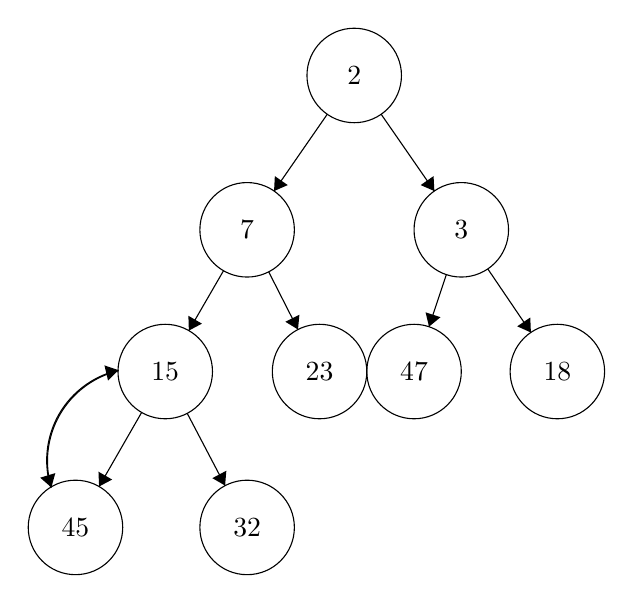
\begin{tikzpicture}[scale=0.2]
\tikzstyle{every node}+=[inner sep=0pt]
\draw [black] (38.6,-6.5) circle (3);
\draw (38.6,-6.5) node {$2$};
\draw [black] (31.8,-16.3) circle (3);
\draw (31.8,-16.3) node {$7$};
\draw [black] (45.4,-16.3) circle (3);
\draw (45.4,-16.3) node {$3$};
\draw [black] (26.6,-25.3) circle (3);
\draw (26.6,-25.3) node {$15$};
\draw [black] (36.4,-25.3) circle (3);
\draw (36.4,-25.3) node {$23$};
\draw [black] (42.4,-25.3) circle (3);
\draw (42.4,-25.3) node {$47$};
\draw [black] (51.5,-25.3) circle (3);
\draw (51.5,-25.3) node {$18$};
\draw [black] (20.9,-35.2) circle (3);
\draw (20.9,-35.2) node {$45$};
\draw [black] (31.8,-35.2) circle (3);
\draw (31.8,-35.2) node {$32$};
\draw [black] (40.31,-8.96) -- (43.69,-13.84);
\fill [black] (43.69,-13.84) -- (43.64,-12.89) -- (42.82,-13.46);
\draw [black] (33.17,-18.97) -- (35.03,-22.63);
\fill [black] (35.03,-22.63) -- (35.12,-21.69) -- (34.23,-22.14);
\draw [black] (44.45,-19.15) -- (43.35,-22.45);
\fill [black] (43.35,-22.45) -- (44.08,-21.85) -- (43.13,-21.54);
\draw [black] (19.366,-32.66) arc (-163.44288:-256.42014:5.896);
\fill [black] (19.37,-32.66) -- (19.62,-31.75) -- (18.66,-32.04);
\draw [black] (28,-27.96) -- (30.4,-32.54);
\fill [black] (30.4,-32.54) -- (30.48,-31.6) -- (29.59,-32.07);
\draw [black] (47.08,-18.78) -- (49.82,-22.82);
\fill [black] (49.82,-22.82) -- (49.78,-21.87) -- (48.95,-22.43);
\draw [black] (36.89,-8.96) -- (33.51,-13.84);
\fill [black] (33.51,-13.84) -- (34.38,-13.46) -- (33.56,-12.89);
\draw [black] (30.3,-18.9) -- (28.1,-22.7);
\fill [black] (28.1,-22.7) -- (28.93,-22.26) -- (28.07,-21.76);
\draw [black] (19.336,-32.678) arc (-162.80965:-257.05337:5.877);
\fill [black] (23.63,-25.21) -- (22.74,-24.91) -- (22.97,-25.88);
\draw [black] (25.1,-27.9) -- (22.4,-32.6);
\fill [black] (22.4,-32.6) -- (23.23,-32.16) -- (22.36,-31.66);
\end{tikzpicture}

This is the final min-heap with the bottom up method. Each node must be compared to its two daughter nodes so total comparisons made = 8 
\end{center}

\pagebreak

\subsection{Min-Heap Top Down}

\begin{center}
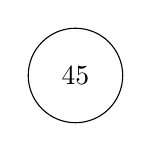
\begin{tikzpicture}[scale=0.2]
\tikzstyle{every node}+=[inner sep=0pt]
\draw [black] (38.6,-6.5) circle (3);
\draw (38.6,-6.5) node {$45$};
\end{tikzpicture}

$\downarrow$
\end{center}

\begin{center}
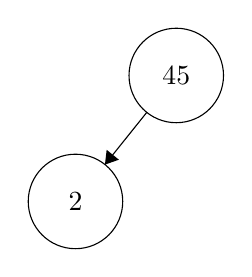
\begin{tikzpicture}[scale=0.2]
\tikzstyle{every node}+=[inner sep=0pt]
\draw [black] (38.6,-6.5) circle (3);
\draw (38.6,-6.5) node {$45$};
\draw [black] (32.2,-14.5) circle (3);
\draw (32.2,-14.5) node {$2$};
\draw [black] (36.73,-8.84) -- (34.07,-12.16);
\fill [black] (34.07,-12.16) -- (34.96,-11.85) -- (34.18,-11.22);
\end{tikzpicture}

$\downarrow$
\end{center}

\begin{center}
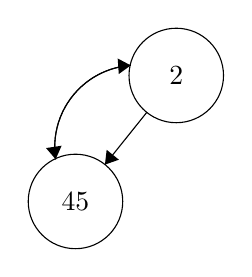
\begin{tikzpicture}[scale=0.2]
\tikzstyle{every node}+=[inner sep=0pt]
\draw [black] (38.6,-6.5) circle (3);
\draw (38.6,-6.5) node {$2$};
\draw [black] (32.2,-14.5) circle (3);
\draw (32.2,-14.5) node {$45$};
\draw [black] (30.941,-11.823) arc (-171.35543:-265.96418:5.195);
\fill [black] (30.94,-11.82) -- (31.32,-10.96) -- (30.33,-11.11);
\draw [black] (30.941,-11.823) arc (-171.36095:-265.95867:5.196);
\fill [black] (35.71,-5.86) -- (34.88,-5.42) -- (34.95,-6.41);
\draw [black] (36.73,-8.84) -- (34.07,-12.16);
\fill [black] (34.07,-12.16) -- (34.96,-11.85) -- (34.18,-11.22);
\end{tikzpicture}

$\downarrow$
\end{center}

\begin{center}
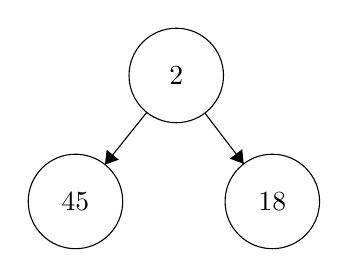
\begin{tikzpicture}[scale=0.2]
\tikzstyle{every node}+=[inner sep=0pt]
\draw [black] (38.6,-6.5) circle (3);
\draw (38.6,-6.5) node {$2$};
\draw [black] (32.2,-14.5) circle (3);
\draw (32.2,-14.5) node {$45$};
\draw [black] (44.7,-14.5) circle (3);
\draw (44.7,-14.5) node {$18$};
\draw [black] (36.73,-8.84) -- (34.07,-12.16);
\fill [black] (34.07,-12.16) -- (34.96,-11.85) -- (34.18,-11.22);
\draw [black] (40.42,-8.89) -- (42.88,-12.11);
\fill [black] (42.88,-12.11) -- (42.79,-11.18) -- (42,-11.78);
\end{tikzpicture}

$\downarrow$
\end{center}

\begin{center}
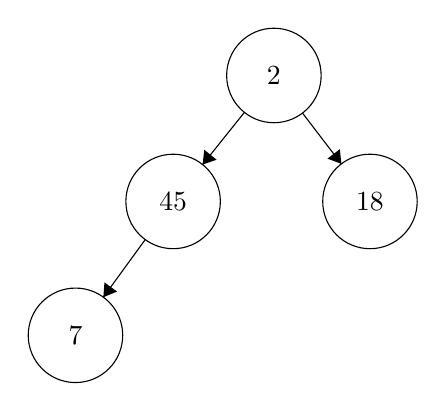
\begin{tikzpicture}[scale=0.2]
\tikzstyle{every node}+=[inner sep=0pt]
\draw [black] (38.6,-6.5) circle (3);
\draw (38.6,-6.5) node {$2$};
\draw [black] (32.2,-14.5) circle (3);
\draw (32.2,-14.5) node {$45$};
\draw [black] (44.7,-14.5) circle (3);
\draw (44.7,-14.5) node {$18$};
\draw [black] (26,-23) circle (3);
\draw (26,-23) node {$7$};
\draw [black] (36.73,-8.84) -- (34.07,-12.16);
\fill [black] (34.07,-12.16) -- (34.96,-11.85) -- (34.18,-11.22);
\draw [black] (40.42,-8.89) -- (42.88,-12.11);
\fill [black] (42.88,-12.11) -- (42.79,-11.18) -- (42,-11.78);
\draw [black] (30.43,-16.92) -- (27.77,-20.58);
\fill [black] (27.77,-20.58) -- (28.64,-20.22) -- (27.84,-19.64);
\end{tikzpicture}

$\downarrow$
\end{center}

\begin{center}
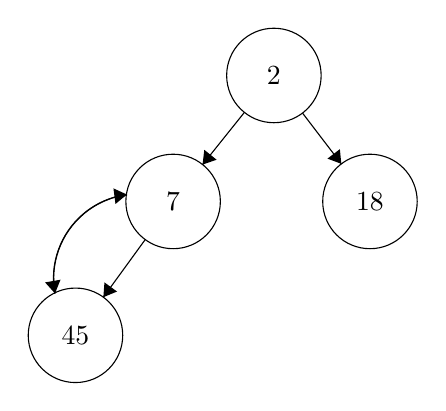
\begin{tikzpicture}[scale=0.2]
\tikzstyle{every node}+=[inner sep=0pt]
\draw [black] (38.6,-6.5) circle (3);
\draw (38.6,-6.5) node {$2$};
\draw [black] (32.2,-14.5) circle (3);
\draw (32.2,-14.5) node {$7$};
\draw [black] (44.7,-14.5) circle (3);
\draw (44.7,-14.5) node {$18$};
\draw [black] (26,-23) circle (3);
\draw (26,-23) node {$45$};
\draw [black] (36.73,-8.84) -- (34.07,-12.16);
\fill [black] (34.07,-12.16) -- (34.96,-11.85) -- (34.18,-11.22);
\draw [black] (40.42,-8.89) -- (42.88,-12.11);
\fill [black] (42.88,-12.11) -- (42.79,-11.18) -- (42,-11.78);
\draw [black] (24.698,-20.34) arc (-169.90444:-262.31046:5.374);
\fill [black] (24.7,-20.34) -- (25.05,-19.47) -- (24.07,-19.64);
\draw [black] (24.687,-20.346) arc (-169.67467:-262.54023:5.369);
\fill [black] (29.27,-14.06) -- (28.41,-13.67) -- (28.54,-14.66);
\draw [black] (30.43,-16.92) -- (27.77,-20.58);
\fill [black] (27.77,-20.58) -- (28.64,-20.22) -- (27.84,-19.64);
\end{tikzpicture}

$\downarrow$
\end{center}

\begin{center}
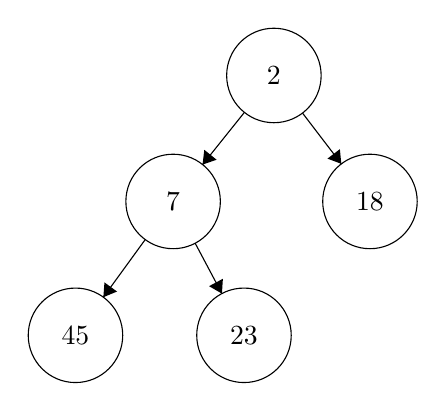
\begin{tikzpicture}[scale=0.2]
\tikzstyle{every node}+=[inner sep=0pt]
\draw [black] (38.6,-6.5) circle (3);
\draw (38.6,-6.5) node {$2$};
\draw [black] (32.2,-14.5) circle (3);
\draw (32.2,-14.5) node {$7$};
\draw [black] (44.7,-14.5) circle (3);
\draw (44.7,-14.5) node {$18$};
\draw [black] (26,-23) circle (3);
\draw (26,-23) node {$45$};
\draw [black] (36.7,-23) circle (3);
\draw (36.7,-23) node {$23$};
\draw [black] (36.73,-8.84) -- (34.07,-12.16);
\fill [black] (34.07,-12.16) -- (34.96,-11.85) -- (34.18,-11.22);
\draw [black] (40.42,-8.89) -- (42.88,-12.11);
\fill [black] (42.88,-12.11) -- (42.79,-11.18) -- (42,-11.78);
\draw [black] (30.43,-16.92) -- (27.77,-20.58);
\fill [black] (27.77,-20.58) -- (28.64,-20.22) -- (27.84,-19.64);
\draw [black] (33.6,-17.15) -- (35.3,-20.35);
\fill [black] (35.3,-20.35) -- (35.36,-19.41) -- (34.48,-19.88);
\end{tikzpicture}

$\downarrow$
\end{center}

\begin{center}
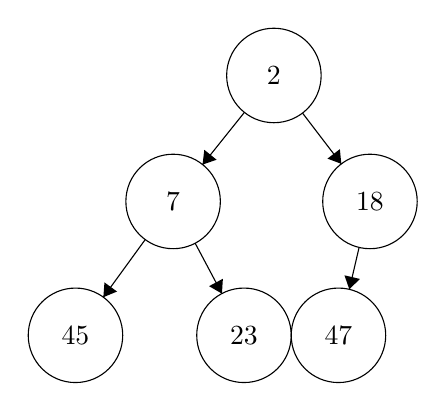
\begin{tikzpicture}[scale=0.2]
\tikzstyle{every node}+=[inner sep=0pt]
\draw [black] (38.6,-6.5) circle (3);
\draw (38.6,-6.5) node {$2$};
\draw [black] (32.2,-14.5) circle (3);
\draw (32.2,-14.5) node {$7$};
\draw [black] (44.7,-14.5) circle (3);
\draw (44.7,-14.5) node {$18$};
\draw [black] (26,-23) circle (3);
\draw (26,-23) node {$45$};
\draw [black] (36.7,-23) circle (3);
\draw (36.7,-23) node {$23$};
\draw [black] (42.7,-23) circle (3);
\draw (42.7,-23) node {$47$};
\draw [black] (36.73,-8.84) -- (34.07,-12.16);
\fill [black] (34.07,-12.16) -- (34.96,-11.85) -- (34.18,-11.22);
\draw [black] (40.42,-8.89) -- (42.88,-12.11);
\fill [black] (42.88,-12.11) -- (42.79,-11.18) -- (42,-11.78);
\draw [black] (30.43,-16.92) -- (27.77,-20.58);
\fill [black] (27.77,-20.58) -- (28.64,-20.22) -- (27.84,-19.64);
\draw [black] (33.6,-17.15) -- (35.3,-20.35);
\fill [black] (35.3,-20.35) -- (35.36,-19.41) -- (34.48,-19.88);
\draw [black] (44.01,-17.42) -- (43.39,-20.08);
\fill [black] (43.39,-20.08) -- (44.06,-19.42) -- (43.08,-19.19);
\end{tikzpicture}

$\downarrow$
\end{center}

\begin{center}
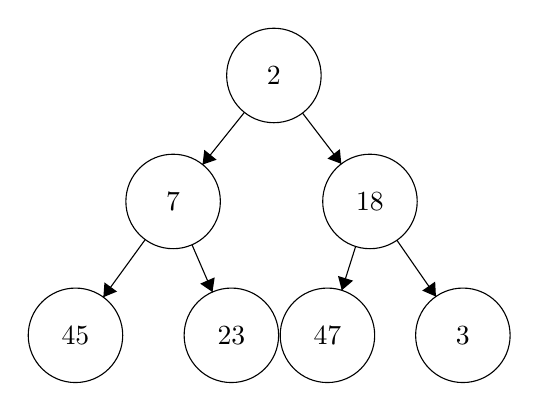
\begin{tikzpicture}[scale=0.2]
\tikzstyle{every node}+=[inner sep=0pt]
\draw [black] (38.6,-6.5) circle (3);
\draw (38.6,-6.5) node {$2$};
\draw [black] (32.2,-14.5) circle (3);
\draw (32.2,-14.5) node {$7$};
\draw [black] (44.7,-14.5) circle (3);
\draw (44.7,-14.5) node {$18$};
\draw [black] (26,-23) circle (3);
\draw (26,-23) node {$45$};
\draw [black] (35.9,-23) circle (3);
\draw (35.9,-23) node {$23$};
\draw [black] (42,-23) circle (3);
\draw (42,-23) node {$47$};
\draw [black] (50.6,-23) circle (3);
\draw (50.6,-23) node {$3$};
\draw [black] (36.73,-8.84) -- (34.07,-12.16);
\fill [black] (34.07,-12.16) -- (34.96,-11.85) -- (34.18,-11.22);
\draw [black] (40.42,-8.89) -- (42.88,-12.11);
\fill [black] (42.88,-12.11) -- (42.79,-11.18) -- (42,-11.78);
\draw [black] (30.43,-16.92) -- (27.77,-20.58);
\fill [black] (27.77,-20.58) -- (28.64,-20.22) -- (27.84,-19.64);
\draw [black] (33.4,-17.25) -- (34.7,-20.25);
\fill [black] (34.7,-20.25) -- (34.84,-19.32) -- (33.92,-19.72);
\draw [black] (43.79,-17.36) -- (42.91,-20.14);
\fill [black] (42.91,-20.14) -- (43.63,-19.53) -- (42.67,-19.23);
\draw [black] (46.41,-16.96) -- (48.89,-20.54);
\fill [black] (48.89,-20.54) -- (48.84,-19.59) -- (48.02,-20.16);
\end{tikzpicture}

$\downarrow$
\end{center}

\begin{center}
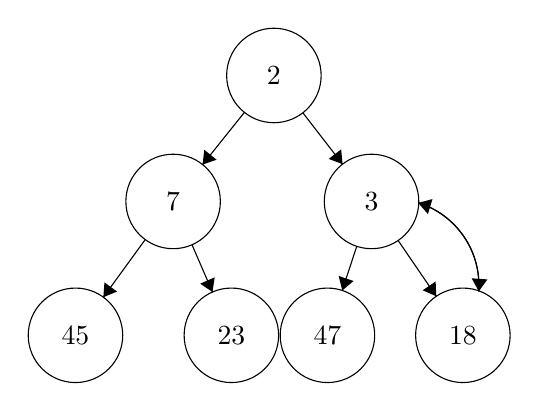
\begin{tikzpicture}[scale=0.2]
\tikzstyle{every node}+=[inner sep=0pt]
\draw [black] (38.6,-6.5) circle (3);
\draw (38.6,-6.5) node {$2$};
\draw [black] (32.2,-14.5) circle (3);
\draw (32.2,-14.5) node {$7$};
\draw [black] (44.8,-14.5) circle (3);
\draw (44.8,-14.5) node {$3$};
\draw [black] (26,-23) circle (3);
\draw (26,-23) node {$45$};
\draw [black] (35.9,-23) circle (3);
\draw (35.9,-23) node {$23$};
\draw [black] (42,-23) circle (3);
\draw (42,-23) node {$47$};
\draw [black] (50.6,-23) circle (3);
\draw (50.6,-23) node {$18$};
\draw [black] (36.73,-8.84) -- (34.07,-12.16);
\fill [black] (34.07,-12.16) -- (34.96,-11.85) -- (34.18,-11.22);
\draw [black] (40.44,-8.87) -- (42.96,-12.13);
\fill [black] (42.96,-12.13) -- (42.87,-11.19) -- (42.08,-11.8);
\draw [black] (30.43,-16.92) -- (27.77,-20.58);
\fill [black] (27.77,-20.58) -- (28.64,-20.22) -- (27.84,-19.64);
\draw [black] (33.4,-17.25) -- (34.7,-20.25);
\fill [black] (34.7,-20.25) -- (34.84,-19.32) -- (33.92,-19.72);
\draw [black] (43.86,-17.35) -- (42.94,-20.15);
\fill [black] (42.94,-20.15) -- (43.66,-19.55) -- (42.71,-19.23);
\draw [black] (47.762,-14.58) arc (72.77544:-4.15986:5.481);
\fill [black] (51.61,-20.21) -- (52.16,-19.45) -- (51.16,-19.38);
\draw [black] (47.762,-14.585) arc (72.68277:-4.06719:5.486);
\fill [black] (47.76,-14.59) -- (48.38,-15.3) -- (48.67,-14.35);
\draw [black] (46.49,-16.98) -- (48.91,-20.52);
\fill [black] (48.91,-20.52) -- (48.87,-19.58) -- (48.05,-20.14);
\end{tikzpicture}

$\downarrow$
\end{center}

\begin{center}
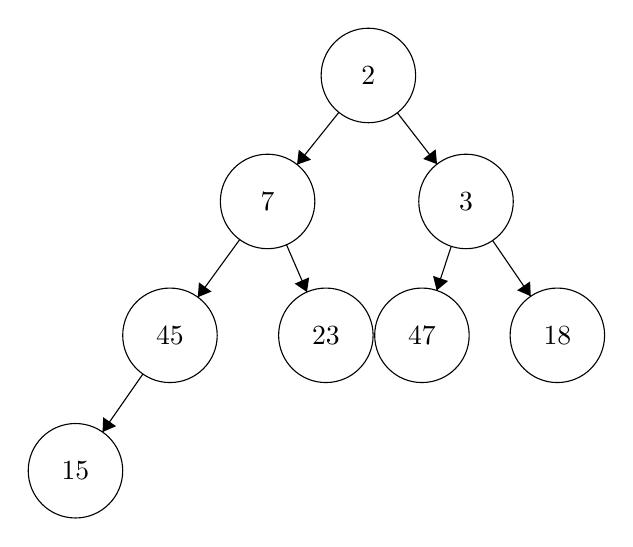
\begin{tikzpicture}[scale=0.2]
\tikzstyle{every node}+=[inner sep=0pt]
\draw [black] (38.6,-6.5) circle (3);
\draw (38.6,-6.5) node {$2$};
\draw [black] (32.2,-14.5) circle (3);
\draw (32.2,-14.5) node {$7$};
\draw [black] (44.8,-14.5) circle (3);
\draw (44.8,-14.5) node {$3$};
\draw [black] (26,-23) circle (3);
\draw (26,-23) node {$45$};
\draw [black] (35.9,-23) circle (3);
\draw (35.9,-23) node {$23$};
\draw [black] (42,-23) circle (3);
\draw (42,-23) node {$47$};
\draw [black] (50.6,-23) circle (3);
\draw (50.6,-23) node {$18$};
\draw [black] (20,-31.6) circle (3);
\draw (20,-31.6) node {$15$};
\draw [black] (36.73,-8.84) -- (34.07,-12.16);
\fill [black] (34.07,-12.16) -- (34.96,-11.85) -- (34.18,-11.22);
\draw [black] (40.44,-8.87) -- (42.96,-12.13);
\fill [black] (42.96,-12.13) -- (42.87,-11.19) -- (42.08,-11.8);
\draw [black] (30.43,-16.92) -- (27.77,-20.58);
\fill [black] (27.77,-20.58) -- (28.64,-20.22) -- (27.84,-19.64);
\draw [black] (33.4,-17.25) -- (34.7,-20.25);
\fill [black] (34.7,-20.25) -- (34.84,-19.32) -- (33.92,-19.72);
\draw [black] (43.86,-17.35) -- (42.94,-20.15);
\fill [black] (42.94,-20.15) -- (43.66,-19.55) -- (42.71,-19.23);
\draw [black] (46.49,-16.98) -- (48.91,-20.52);
\fill [black] (48.91,-20.52) -- (48.87,-19.58) -- (48.05,-20.14);
\draw [black] (24.28,-25.46) -- (21.72,-29.14);
\fill [black] (21.72,-29.14) -- (22.58,-28.77) -- (21.76,-28.2);
\end{tikzpicture}

$\downarrow$
\end{center}

\begin{center}
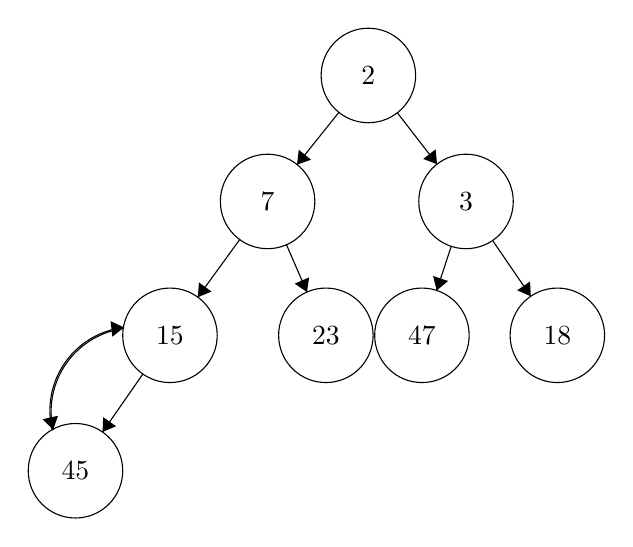
\begin{tikzpicture}[scale=0.2]
\tikzstyle{every node}+=[inner sep=0pt]
\draw [black] (38.6,-6.5) circle (3);
\draw (38.6,-6.5) node {$2$};
\draw [black] (32.2,-14.5) circle (3);
\draw (32.2,-14.5) node {$7$};
\draw [black] (44.8,-14.5) circle (3);
\draw (44.8,-14.5) node {$3$};
\draw [black] (26,-23) circle (3);
\draw (26,-23) node {$15$};
\draw [black] (35.9,-23) circle (3);
\draw (35.9,-23) node {$23$};
\draw [black] (42,-23) circle (3);
\draw (42,-23) node {$47$};
\draw [black] (50.6,-23) circle (3);
\draw (50.6,-23) node {$18$};
\draw [black] (20,-31.6) circle (3);
\draw (20,-31.6) node {$45$};
\draw [black] (36.73,-8.84) -- (34.07,-12.16);
\fill [black] (34.07,-12.16) -- (34.96,-11.85) -- (34.18,-11.22);
\draw [black] (40.44,-8.87) -- (42.96,-12.13);
\fill [black] (42.96,-12.13) -- (42.87,-11.19) -- (42.08,-11.8);
\draw [black] (30.43,-16.92) -- (27.77,-20.58);
\fill [black] (27.77,-20.58) -- (28.64,-20.22) -- (27.84,-19.64);
\draw [black] (33.4,-17.25) -- (34.7,-20.25);
\fill [black] (34.7,-20.25) -- (34.84,-19.32) -- (33.92,-19.72);
\draw [black] (43.86,-17.35) -- (42.94,-20.15);
\fill [black] (42.94,-20.15) -- (43.66,-19.55) -- (42.71,-19.23);
\draw [black] (46.49,-16.98) -- (48.91,-20.52);
\fill [black] (48.91,-20.52) -- (48.87,-19.58) -- (48.05,-20.14);
\draw [black] (18.578,-29.003) arc (-167.42176:-262.38323:5.328);
\fill [black] (18.58,-29) -- (18.89,-28.11) -- (17.92,-28.33);
\draw [black] (18.526,-29.033) arc (-166.32286:-263.48213:5.309);
\fill [black] (23.08,-22.5) -- (22.23,-22.1) -- (22.34,-23.09);
\draw [black] (24.28,-25.46) -- (21.72,-29.14);
\fill [black] (21.72,-29.14) -- (22.58,-28.77) -- (21.76,-28.2);
\end{tikzpicture}

$\downarrow$
\end{center}

\begin{center}
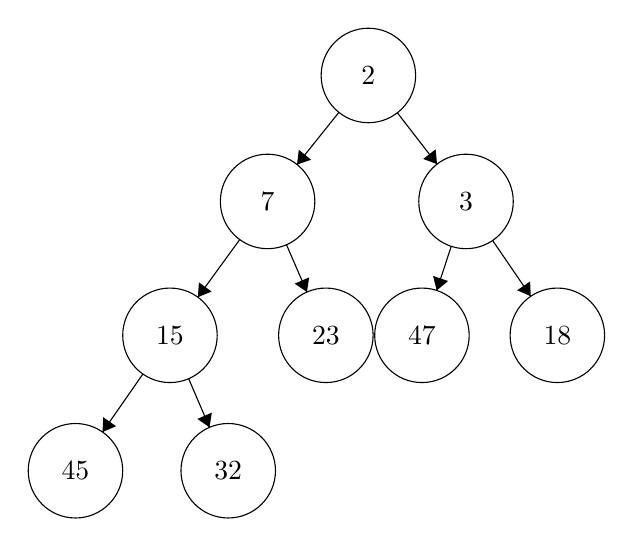
\begin{tikzpicture}[scale=0.2]
\tikzstyle{every node}+=[inner sep=0pt]
\draw [black] (38.6,-6.5) circle (3);
\draw (38.6,-6.5) node {$2$};
\draw [black] (32.2,-14.5) circle (3);
\draw (32.2,-14.5) node {$7$};
\draw [black] (44.8,-14.5) circle (3);
\draw (44.8,-14.5) node {$3$};
\draw [black] (26,-23) circle (3);
\draw (26,-23) node {$15$};
\draw [black] (35.9,-23) circle (3);
\draw (35.9,-23) node {$23$};
\draw [black] (42,-23) circle (3);
\draw (42,-23) node {$47$};
\draw [black] (50.6,-23) circle (3);
\draw (50.6,-23) node {$18$};
\draw [black] (20,-31.6) circle (3);
\draw (20,-31.6) node {$45$};
\draw [black] (29.7,-31.6) circle (3);
\draw (29.7,-31.6) node {$32$};
\draw [black] (36.73,-8.84) -- (34.07,-12.16);
\fill [black] (34.07,-12.16) -- (34.96,-11.85) -- (34.18,-11.22);
\draw [black] (40.44,-8.87) -- (42.96,-12.13);
\fill [black] (42.96,-12.13) -- (42.87,-11.19) -- (42.08,-11.8);
\draw [black] (30.43,-16.92) -- (27.77,-20.58);
\fill [black] (27.77,-20.58) -- (28.64,-20.22) -- (27.84,-19.64);
\draw [black] (33.4,-17.25) -- (34.7,-20.25);
\fill [black] (34.7,-20.25) -- (34.84,-19.32) -- (33.92,-19.72);
\draw [black] (43.86,-17.35) -- (42.94,-20.15);
\fill [black] (42.94,-20.15) -- (43.66,-19.55) -- (42.71,-19.23);
\draw [black] (46.49,-16.98) -- (48.91,-20.52);
\fill [black] (48.91,-20.52) -- (48.87,-19.58) -- (48.05,-20.14);
\draw [black] (24.28,-25.46) -- (21.72,-29.14);
\fill [black] (21.72,-29.14) -- (22.58,-28.77) -- (21.76,-28.2);
\draw [black] (27.19,-25.76) -- (28.51,-28.84);
\fill [black] (28.51,-28.84) -- (28.66,-27.91) -- (27.74,-28.31);
\end{tikzpicture}

This is the final min-heap with the Top Down method. Each node must be compared to its two daughter nodes so total comparisons made = 8 
\end{center}

\pagebreak

\subsection{Analysis}

Yes, the two heaps are identical in the end. I don't believe this is just a peculiar case where both heaps end up exactly the same. Since we are starting with the data in the same order in each case: 45, 2, 18, 7, 23, 47, 3, 15, 32, the resulting construction will be the same no matter which method is used because the comparisons are carried out on the same values just with different core methods. If however the order of the incoming data was swapped, e.g. 2, 3, 45, 7, 32, 15, 47, 18, 23. The resultant min-heap would be different than with the original incoming data set. However both Bottom up and Top down would again produce the same heaps on the new set.

\pagebreak

\section{Fake Coin}

In order to find the asymptotic lower bound for which of the coins is fake, we need to look at an $f(n)$, that regardless of the algorithm used to produce the correct answer, will take a minimum of $f(n)$ weighings to do. Hypothetically, if you select just two coins from the collection and weight them against each other and one is lighter than the other. Then you have found the fake coin in the minimum number of steps possible, but you still needed 1 weighing to do so. So no matter which method you use to uncover the fake coin, it will require 1 weighing and thus a lower bound is $\Omega(1)$.

\begin{center}
\begin{tikzpicture}[scale=0.2]
\tikzstyle{every node}+=[inner sep=0pt]
\draw [black] (38.6,-6.3) circle (3);
\draw (38.6,-6.3) node {$n_{1}$};
\draw [black] (48.6,-21) circle (3);
\draw (48.6,-21) node {$n_{3}$};
\draw [black] (28.1,-21) circle (3);
\draw (28.1,-21) node {$n_{1} \neq n_{2}$};
\draw [black] (41.8,-34.7) circle (3);
\draw (41.8,-34.7) node {$n_{3} \neq n_{4}$};
\draw [black] (56.7,-34.7) circle (3);
\draw (56.7,-34.7) node {$n_{5}$};
\draw [black] (40.29,-8.78) -- (46.91,-18.52);
\fill [black] (46.91,-18.52) -- (46.88,-17.58) -- (46.05,-18.14);
\draw [black] (36.86,-8.74) -- (29.84,-18.56);
\fill [black] (29.84,-18.56) -- (30.72,-18.2) -- (29.9,-17.62);
\draw [black] (47.27,-23.69) -- (43.13,-32.01);
\fill [black] (43.13,-32.01) -- (43.94,-31.52) -- (43.04,-31.07);
\draw [black] (50.13,-23.58) -- (55.17,-32.12);
\fill [black] (55.17,-32.12) -- (55.2,-31.17) -- (54.34,-31.68);
\end{tikzpicture}
\end{center}

When you select two coins, and weigh them, you only have two options, they weigh the same or not, if they weigh the same, select another 2 coins and repeat. (Note: this method is far inferior to the grouping method, it would take at worst case $\frac{n}{2}$ weighings to find the fake coin as opposed to $log(n)$, it was used just to illustrate a point). So the best case for any method would also require at minimum 1 weighing.



\end{document}
%%%%%%%%%%%%%%%%%%%%%%%%%%%%%%%%%%%%%%%%%%%%%%%%%%%%%%%%%%%%%%%%%%%%%%

